\section{Breath-First and Depth-First Search}
Two general methods for traversing a graph are, \textbf{breadth-first search} and \textbf{depth-first search}.

\begin{Def}[Cycle]

    A \textbf{cycle} is a path that starts and ends at the same node.
\end{Def}
\textbf{Example:} In the above Figure (\ref{fig:adj_matri_dir}), $1\rightarrow 2 \rightarrow 3 \rightarrow 1$ form a cycle.
\begin{Def}[Tree]

    A \textbf{tree} is a connected graph with no cycles. A \textbf{leaf-nodes} is the outer-most nodes of a tree. A \textbf{branch} is a path from the root to a leaf.  
\end{Def}
\newpage
\begin{theo}[Tree Identity]

    Let $G$ be an undirected graph of $n$ nodes. Then any two statements imply the third:
    \begin{enumerate}
        \item [(i.)] $G$ is connected.
        \item [(ii.)] $G$ has $n-1$ edges.
        \item [(iii.)] $G$ has no cycles.
    \end{enumerate}
\end{theo}

\begin{Def}[Rooted Trees]
    
        Let $T$ be a tree with a designated root node $r$. Then each degree is 
        considered an outdegree, called a \textbf{child}, and its indegree its \textbf{parent}.
\end{Def}
\begin{figure}[h]
    \begin{center}
      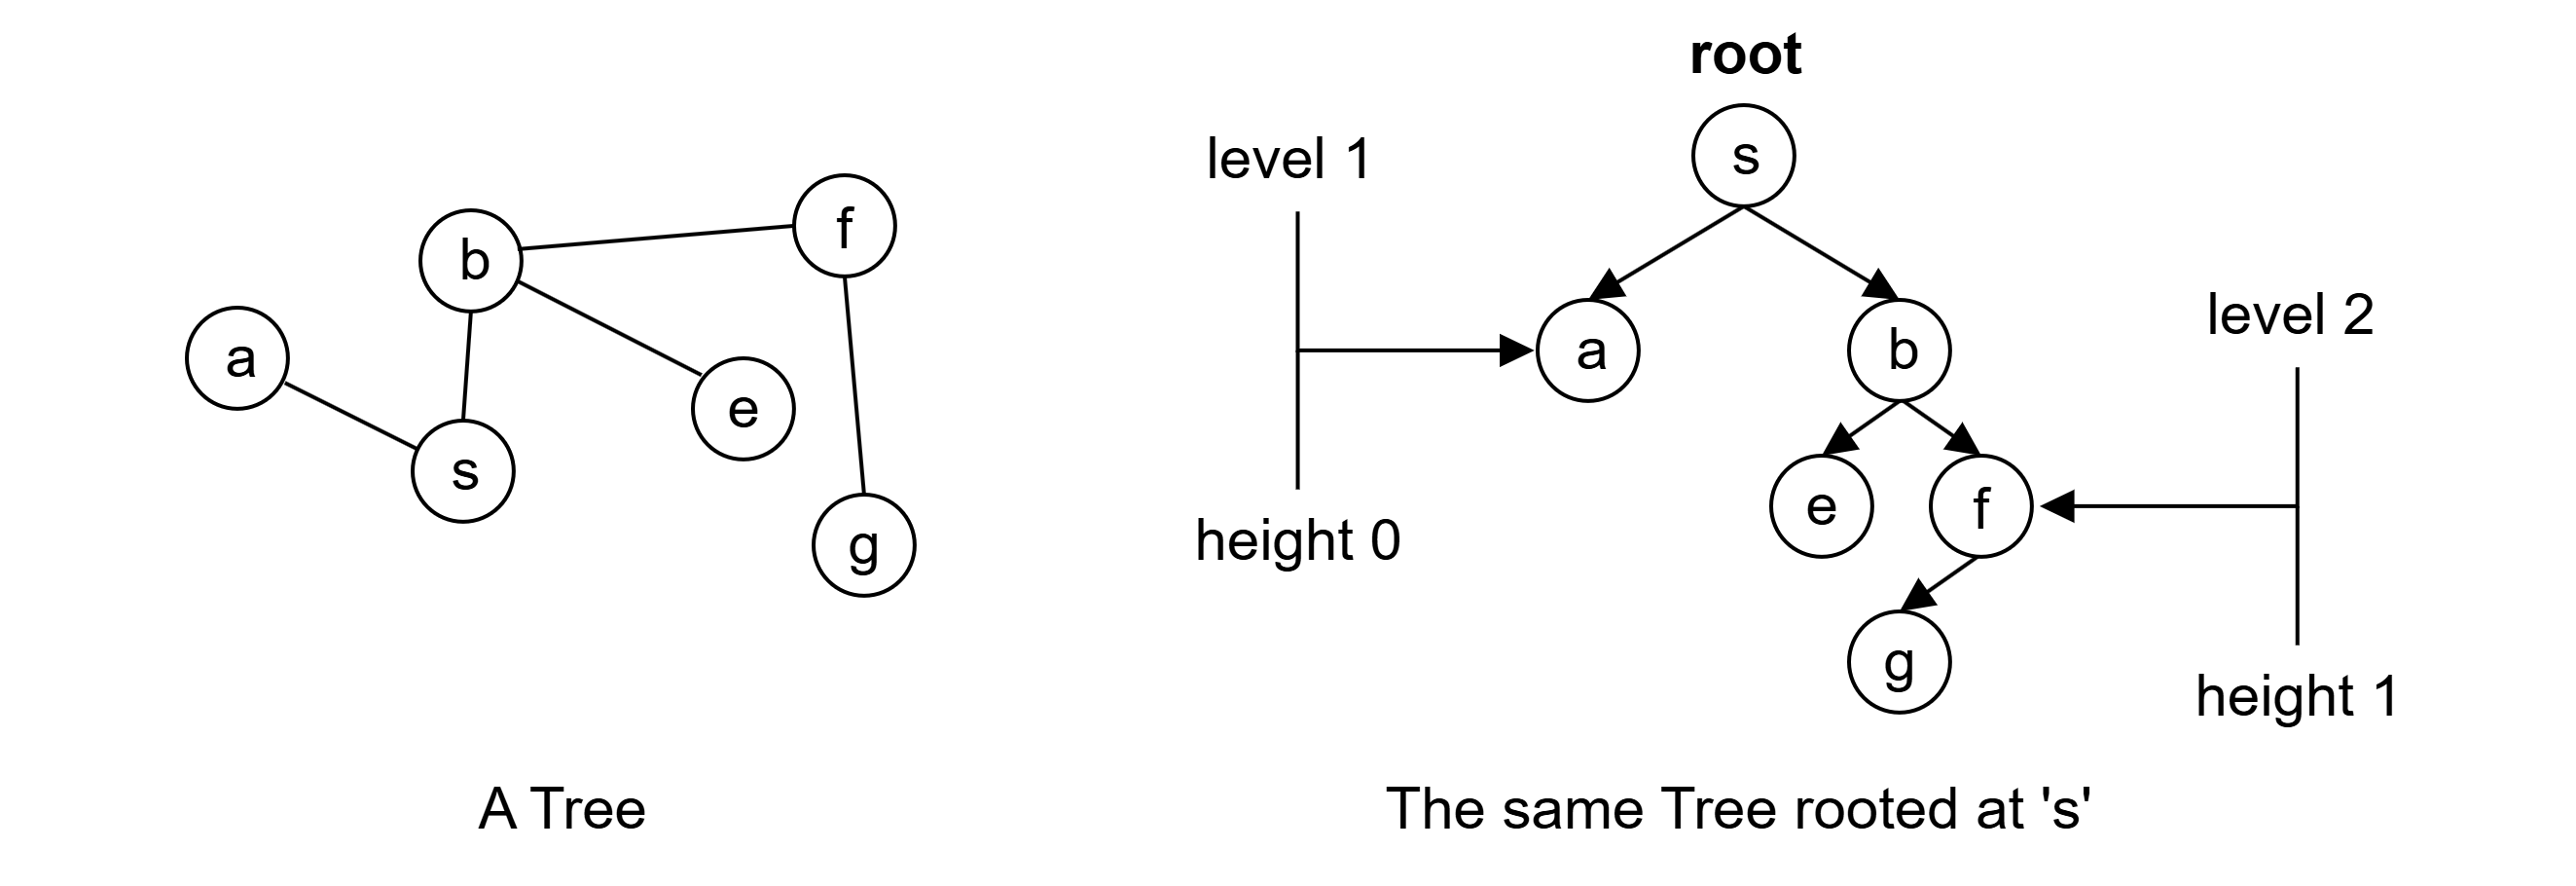
\includegraphics[height=2in]{./Sections/graphs/rooted_tree.png}
    \end{center}
     \caption{A rooted tree with root 1 and children $\{2,5,7\}$}\label{fig:rooted_tree}
  \end{figure}

\begin{Def}[Levels and Heights]

    The \textbf{level} of a node is the number of edges from the root. The \textbf{height} of a tree is the maximum level of any node.
\end{Def}
\textbf{Example:} In Figure (\ref{fig:rooted_tree})'s rooted tree , node 5 has a level of 1, and the height of the tree is 2.
\newpage
\begin{Def}[Breadth-First Search (BFS)]

    In a \textbf{breadth-first search}, we start at a node's children first before moving onto their children's children in level order.
\end{Def}
\begin{figure}[h]
    \begin{center}
      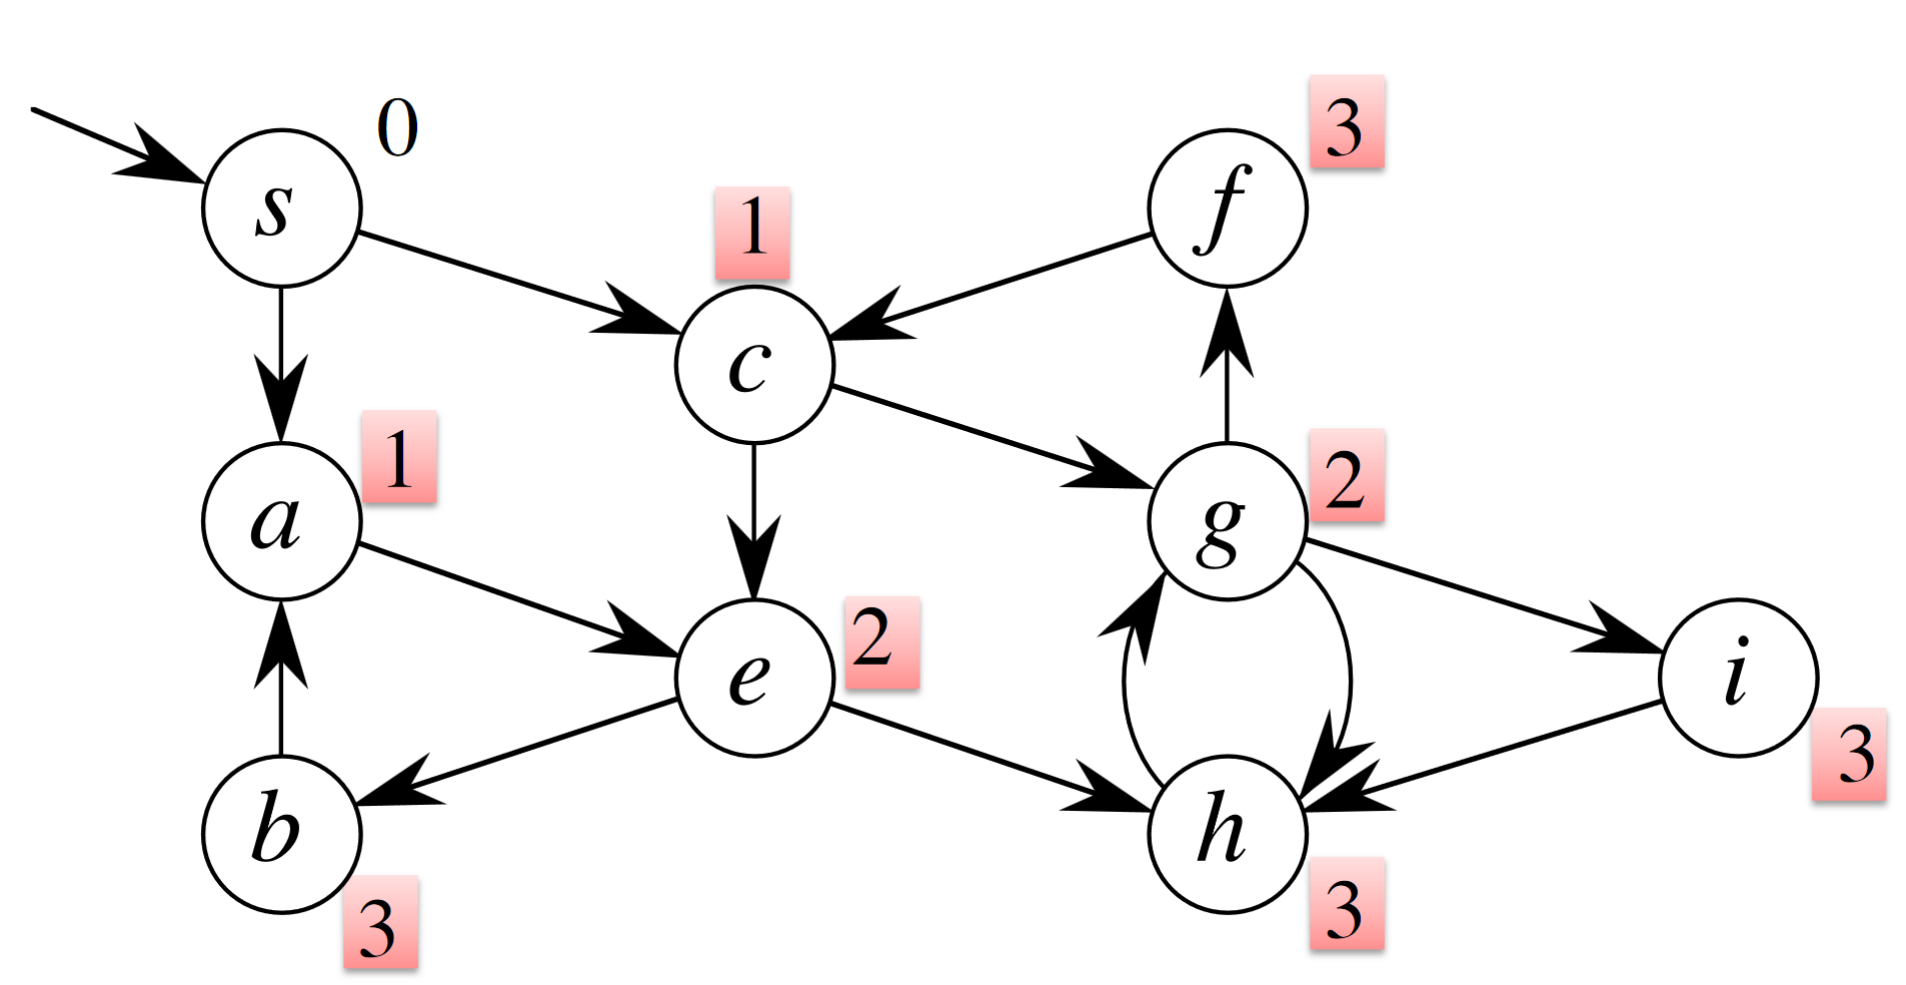
\includegraphics[height=2in]{./Sections/graphs/bfs.png}
    \end{center}
     \caption{A BFS tree traversal preformed on a graph with each level enumerated}\label{fig:bfs}
  \end{figure}

\begin{theo}[Properties of BFS]
    
    BFS run on any graph $T$ produces a tree $T'$ with the following properties:
    \begin{enumerate}
        \item [(i.)] $T'$ is a tree.
        \item [(ii.)] $T'$ is a rooted tree with the starting node as the root.
        \item [(iii.)] The height of $T'$ is the shortest path from the root to any node.
        \item [(iv.)] Any sub-paths of $T'$ are also shortest paths.
    \end{enumerate}
\end{theo}
\begin{Proof}[Proof of BFS]

    (i.) and (ii.) follow from the definition of a tree. (iii.) and (iv.) follow that since a tree 
    contains a direct path to any given node in our parent child relationship, that path must be the shortest.
\end{Proof}
\begin{Tip}
    In a family tree, there is only one path from each ancestor to each descendant.
\end{Tip}

\newpage 

\noindent
We create a BFS algorithm from what we know, though not the best implementation:
\begin{Func}[BFS Algorithm - \texttt{BFS($s$)}]
    Breadth-First Search starting from node $s$.
    
    \vspace{.5em}
    \noindent
    \textbf{Input:} Graph $G = (V, E)$ and starting node $s$.\\
    \textbf{Output:} Levels of each vertex from $s$.\\
    \begin{algorithm}[H]
        \SetAlgoLined
        \SetKwProg{Fn}{Function}{:}{}
        \Fn{\texttt{BFS($s$)}}{
            \For{each $v \in V$}{
                Level[$v$] $\gets \infty$\;
            }
            Level[$s$] $\gets 0$\;
            Add $s$ to $Q$\;
            \While{$Q$ not empty}{
                $u \gets Q$.Dequeue()\;
                \For{each $v \in G[u]$}{
                    \If{Level[$v$] $= \infty$}{
                        Add edge $(u, v)$ to tree $T$ (parent[$v$] $= u$)\;
                        Add $v$ to $Q$\;
                        Level[$v$] $\gets$ Level[$u$] + 1\;
                    }
                }
            }
        }
    \end{algorithm}
\end{Func}
\vspace{-2em}
\begin{figure}[h]
    \begin{center}
      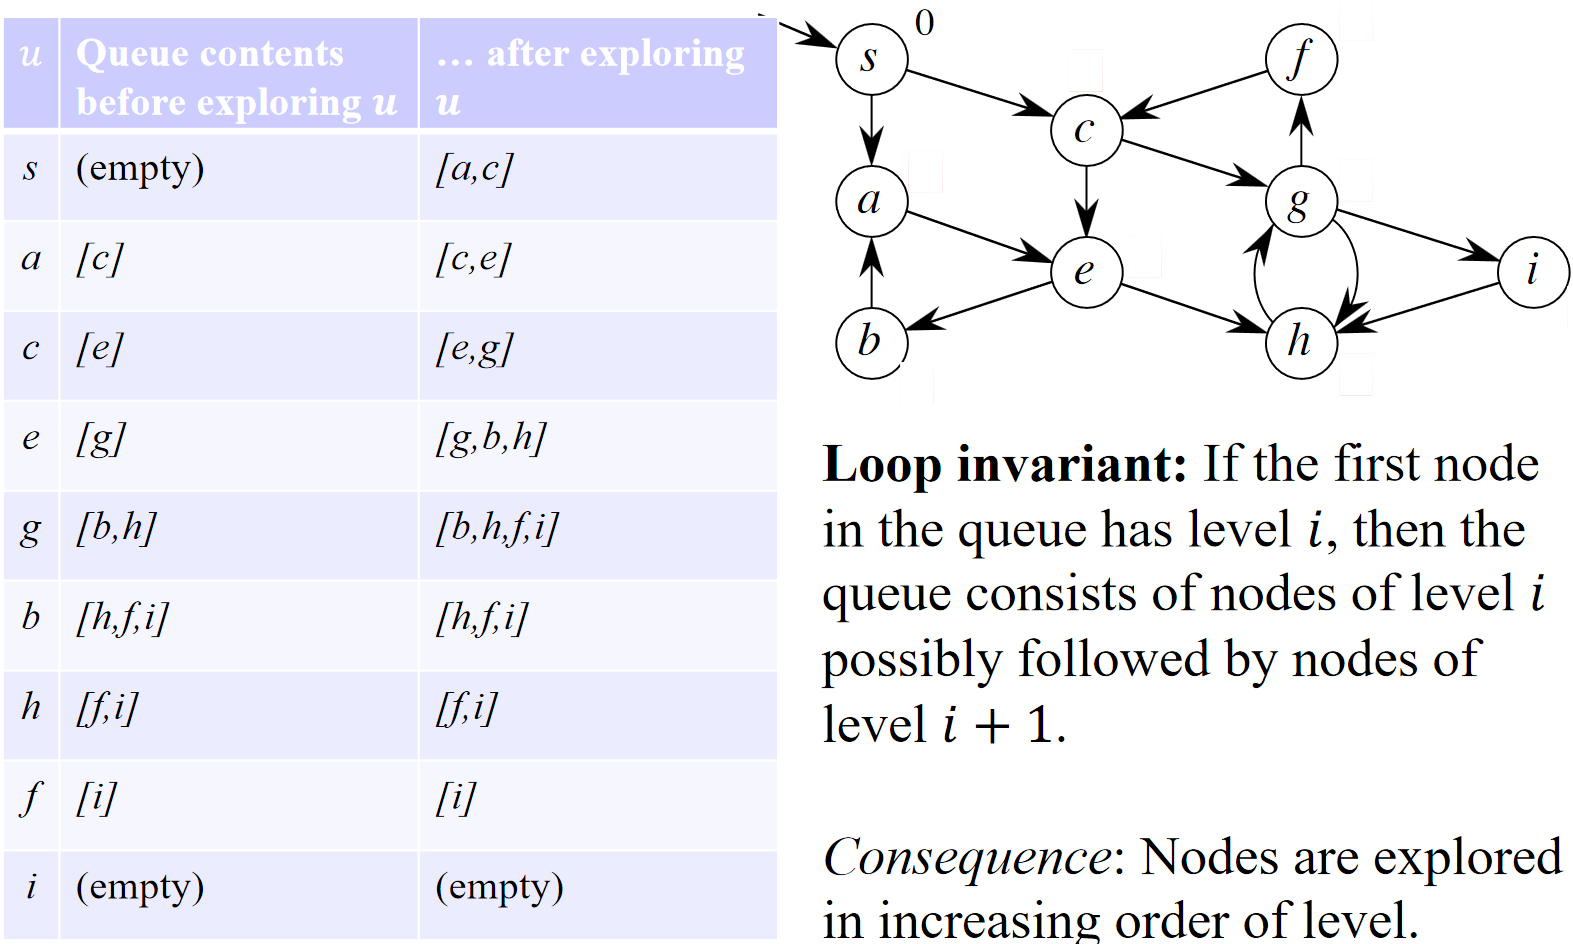
\includegraphics[height=2.9in]{./Sections/graphs/bfs_q.png}
    \end{center}
     \caption{A table showing the queue at each level of iteration}\label{fig:bfs_q}
  \end{figure}

  \newpage

We analyze the time and space complexity in the below Figure (\ref{fig:bfs_q_ana}):

\begin{figure}[h]
    \begin{center}
      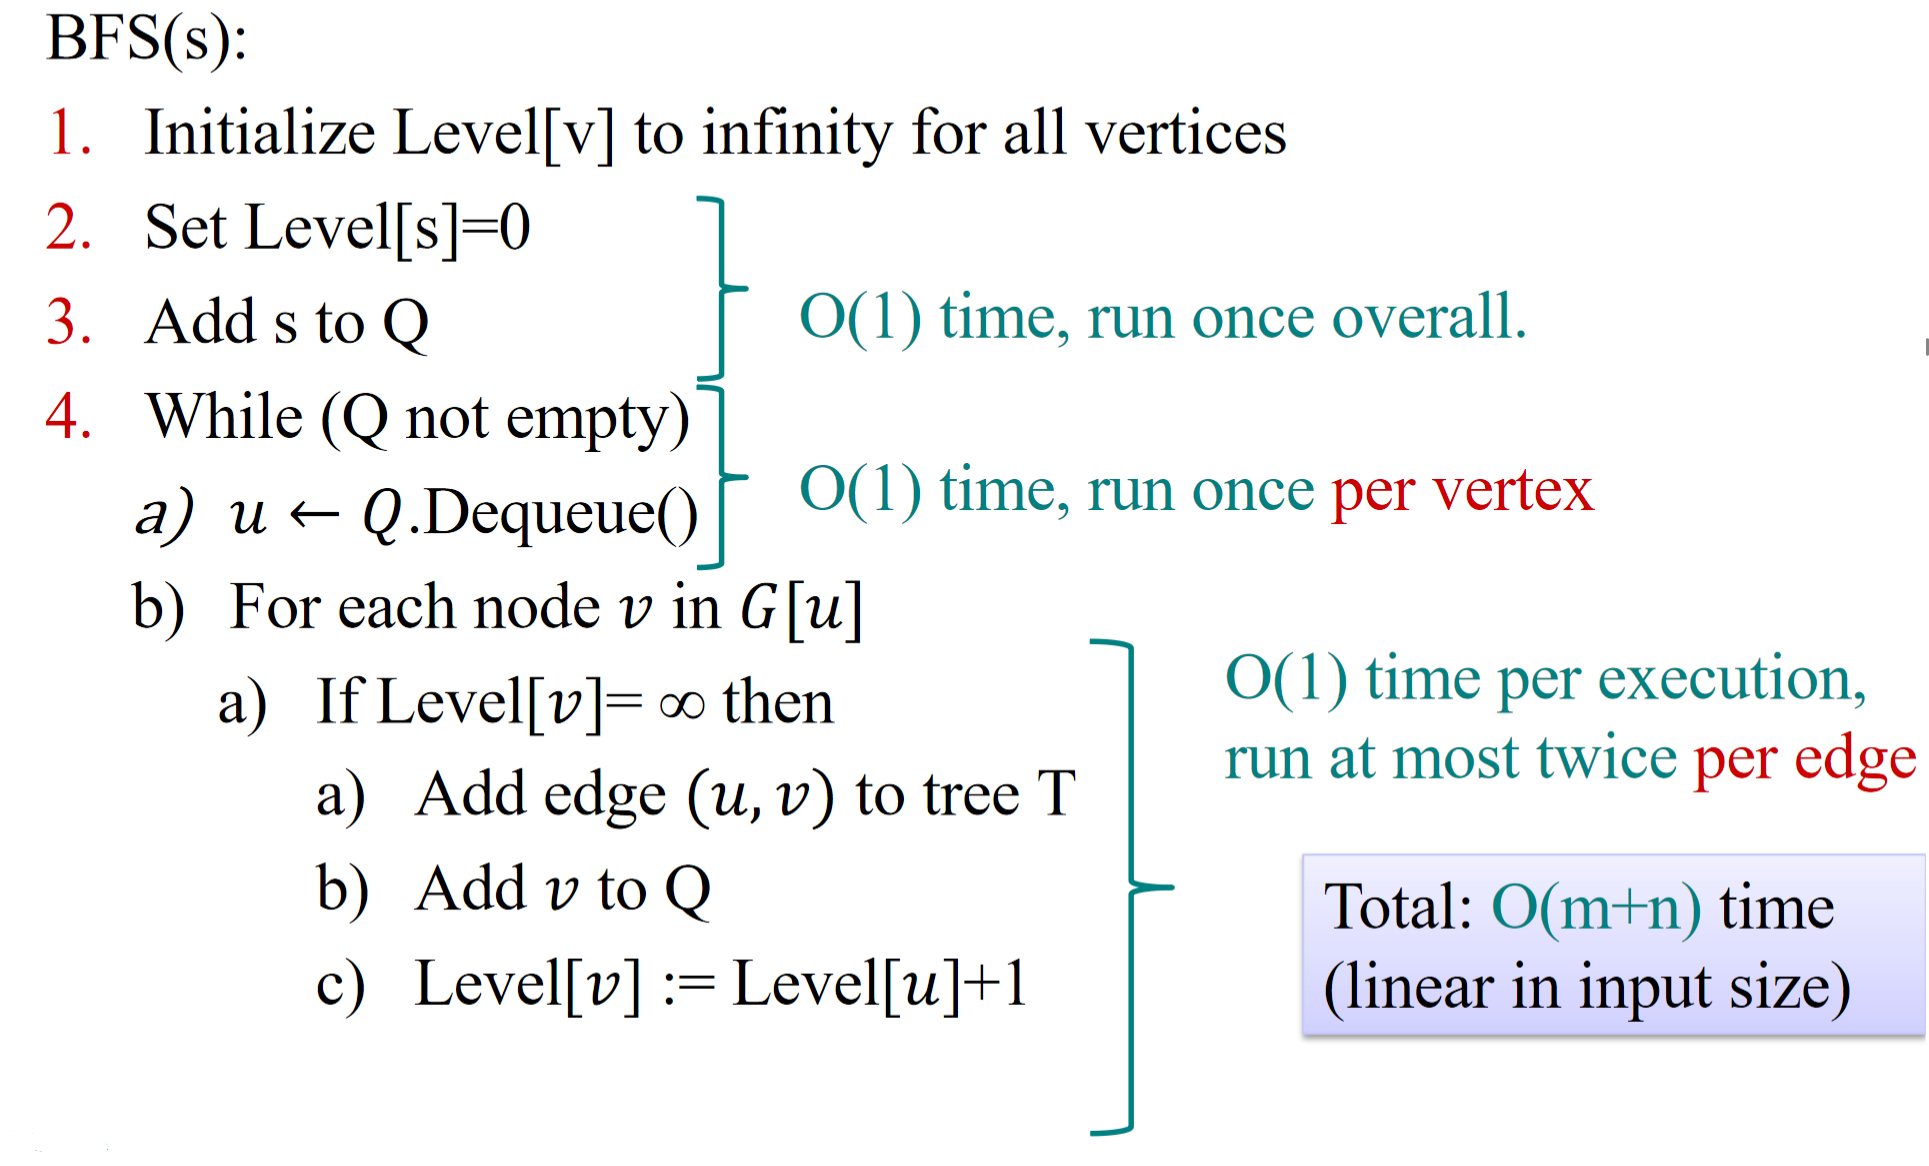
\includegraphics[height=2in]{./Sections/graphs/bfs_q_ana.png}
    \end{center}
     \caption{An analysis showing $O(m+n)$ for both time and space complexity}\label{fig:bfs_q_ana}
  \end{figure}
  \begin{Proof}[Claim 1 for BFS]
    Let $s$ be the root of the BFS tree, then:
    \textbf{Proof:} Induction on the distance from $s$ to $u$.
    
    \textbf{Base case} ($u = s$): The code sets Level[$s$] = 0, and there is no path to find since the path has length 0.
    
    \textbf{Induction hypothesis:} For every node $u$ at distance $\leq i$, Claim 1 holds.
    
    \textbf{Induction step:}
    \begin{itemize}
        \item Let $v$ be a node at distance exactly $i + 1$ from $s$. Let $u$ be its parent in the BFS tree.
        \item The code sets Level[$v$] = Level[$u$] + 1.
        \item Let $x$ be the last node before $v$ on a shortest path from $s$ to $v$. Since $v$ is at distance $i + 1$, then $x$ must be at distance $i$, and so Level[$x$] = $i$ (by induction hypothesis).
        \item If $u = x$, we are done!
        \item If $u \neq x$, then it must be that $u$ was explored before $x$, since otherwise $x$ would be the parent of $u$.
        \item Since we explore nodes in order of level, Level[$u$] $\leq$ Level[$x$] = $i$.
        \item If Level[$u$] = $i$, then we are done.
        \item If Level[$u$] $<$ $i$, then the path $s \sim u \to v$ has length at most $i$, which contradicts the assumption that the distance of $v$ is $i + 1$.
    \end{itemize}
    
    We conclude that Level[$u$] = $i$, Level[$v$] = $i + 1$, and the path in the BFS tree that goes from $s$ to $u$ to $v$ has length $i + 1$. QED.
    \end{Proof}
    
    \newpage

    \begin{Def}[Tyes of Edges]

        In graphs we have three types of edges:
        \begin{enumerate}
            \item \textbf{Tree-edges:} An Edge present in a BFS tree.
            \item \textbf{Forward-edges:} Edges from an ancestor to a descendant.
            \item \textbf{Back-edges:} Edges from a descendant to an ancestor.
            \item \textbf{Cross-edges:} Edges between which connect nodes that have no ancestor-descendant relationship.
        \end{enumerate}
    \end{Def}

    \noindent
    \textbf{Example:} In Figure (\ref{fig:bfs}), $\{(s,c),(a,c),...\}$ are forward and tree edges, $\{(g,h)\}$ are cross edges.\\

    \noindent
    The following arises from the above definitions:
    \begin{theo}[BFS does not Contain Back-edges]
        
        In a BFS tree, there are no back-edges, as they would create a cycle.
    \end{theo}
    \begin{Note}
        \textbf{Note:} In Figure (\ref{fig:bfs}), $b\rightarrow a$ is not a tree-edge, $a$ is on level 1 and $b$ on level 3. If
        this connection were to occur, it would create a cycle, breaking our tree.
    \end{Note}
    \newpage
    \begin{Def}[Depth-First Search (DFS)]

        In a \textbf{depth-first search}, we recursively explore each an entire branch before moving onto the next.
    \end{Def}

    \begin{Func}[DFS Algorithm - \texttt{DFS($G$)}]
        Depth-First Search on graph $G$ (recursive).
    
        \vspace{.5em}
        \noindent
        \textbf{Input:} Graph $G = (V, E)$.\\
        \textbf{Output:} Discovery and finishing times for each vertex.
        
        \begin{algorithm}[H]
            \SetAlgoLined
            \SetKwProg{Fn}{Function}{:}{}
            \Fn{\texttt{DFS($G$)}}{
                \For{each $u \in G$}{
                    $u$.state $\gets$ \texttt{unvisited}\;
                }
                time $\gets 0$\;
                \For{each $u \in G$}{
                    \If{$u$.state == \texttt{unvisited}}{
                        \texttt{DFS-Visit($u$)}\;
                    }
                }
            }
            \vspace{.5em}
            \Fn{\texttt{DFS-Visit($u$)}}{
                time $\gets$ time + 1\;
                $u.d \gets$ time \; // record discovery time\;
                $u$.state $\gets$ \texttt{discovered}\;
                \For{each $v \in G[u]$}{
                    \If{$v$.state == \texttt{unvisited}}{
                        \texttt{DFS-Visit($v$)}\;
                    }
                }
                $u$.state $\gets$ \texttt{returned}\;
                time $\gets$ time + 1\;
                $u.f \gets$ time\; // record finishing time\;
            }
        \end{algorithm}

        \noindent
        \textbf{Time and Space Complexity:} $O(n+m)$ where $n$ is the number of vertices and $m$ the number of edges.
    \end{Func}
    